\documentclass[aps,pra,showpacs,reprint,onecolumn,notitlepage]{revtex4-1}

\usepackage{siunitx}
\sisetup{separate-uncertainty}
\usepackage{graphicx}
\usepackage{dcolumn}
\usepackage{bm}
\usepackage{hyperref}
\usepackage{epstopdf}% To incorporate .eps illustrations using PDFLaTeX, etc.
%\usepackage{subfigure}% Support for small, `sub' figures and tables
\usepackage{placeins}
\usepackage{color}
\usepackage{mathtools}

%math
\usepackage{amssymb}
\usepackage{amsmath} %right equation numbering + mathenvironments
\usepackage{bm} 
\renewcommand{\baselinestretch}{1.1}
\usepackage{xfrac} %%\sfrac for 1/2 type fractions

%OWN COMMANDS
\newcommand{\enquoteit}[1]{``#1''}
\newcommand{\avr}[1]{\mathop{\left\langle #1 \right\rangle}\nolimits}
\newcommand{\create}[0]{\mathop{\hat{a}^{\dagger}}\nolimits}
\newcommand{\anihil}[0]{\mathop{\hat{a}^{}}\nolimits}
\newcommand{\bra}[1]{\mathop{\left\langle #1 \right|}\nolimits}
\newcommand{\ket}[1]{\mathop{\left| #1 \right\rangle}\nolimits}
\newcommand{\tx}[1]{\textnormal{#1}}
\def\@fnsymbol#1{\ensuremath{\ifcase#1\or *\or \dagger\or \ddagger\or
   \mathsection\or \mathparagraph\or \|\or **\or \dagger\dagger
   \or \ddagger\ddagger \else\@ctrerr\fi}}
\newcommand{\ssym}[1]{^{\@fnsymbol{#1}}}

\begin{document}

\title{Controlling the spectrum of single photons from\\ triply-resonant parametric down-conversion}
\pdfoutput=1
\author{author, author, ...$^{1,2,*}$}
%\author{Gerhard Schunk$^{1,2,3,*}$}
%\author{Ulrich Vogl$^{1,2}$}
%\author{Florian Sedlmeir$^{1,2,3}$}
%\author{Dmitry V. Strekalov$^{1,2}$}
%\author{Alexander Otterpohl$^{1,2}$}
%\author{Valentin Averchenko$^{1,2,3}$}
%\author{Harald G. L. Schwefel$^{1,2,4}$}
%\author{Gerd Leuchs$^{1,2}$}
%\author{Christoph Marquardt$^{1,2,6}$}
\affiliation{$^{1}$Max Planck Institute for the Science of Light, G\"{u}nther-Scharowsky-Stra\ss e 1/Building 24, 90158 Erlangen, Germany}              
\affiliation{$^{2}$Institute for Optics, Information and Photonics, University Erlangen-N\"{u}rnberg, Staudtstr.7/B2, 90158 Erlangen, Germany}
\affiliation{$^{3}$SAOT, School in Advanced Optical Technologies, Paul-Gordan-Str. 6, 91052 Erlangen, Germany}
%\affiliation{$^{4}$Department of Physics, University of Otago, 730 Cumberland Street, Dunedin 9016, New Zealand}
%\affiliation{$^{5}$Department of Physics, Technical University of Denmark, Fysikvej Building 309, 2800 Lyngby, Denmark}
%\affiliation{$^{*}$Corresponding author: Gerhard.Schunk@mpl.mpg.de}

%%%%%%%%%%%%%%%%%%%%%%%%%%%%%%%%%%%%%%%%%%%%%%%%%%%%%%

\begin{abstract}
Coupling single photons to a single quantum dot is at the hearth of many quantum repeater protocols. The efficient coupling, however, requires single photons in a specifically tailored spectral and temporal mode. We generate photon pairs via parametric down-conversion in a triply-resonant whispering-gallery mode resonator. In the first part of this work, we discuss the influence of the frequency mismatch $\Delta$ of parametric down-conversion on the spectrum of the parametric photons with a continuous wave pump. The signal and idler spectra deviate from a Lorentzian lineshape for a frequency mismatch other than zero.  In the second part, we use pulsed pump to gain control over the temporal mode of the parametric photons. The temporal mode depends again strongly on the frequency mismatch $\Delta$, which we study in terms of the rise time of the signal photon count rate. Our theoretical and experimental results give a tool specifically tailor the spectral, the temporal, and the entanglement properties of the photon pairs from cavity-assisted parametric down-conversion for a whole class of experiments in quantum optics.
\end{abstract}

\maketitle 

\tableofcontents

\section{Introduction}
%* efficient photon atom coupling, cavity-assisted PDC, Lorentzian line shape. Difficulties to lock the cavity below threshold. Additional locking lasers interfere with the detection at the single photon level, extremely high suppression of the locking beam before the detectors required.  
%
%*pulsing allows to control the number of temporal modes \cite{Brecht2015}. Also exponentially rising pulses \cite{Sych2015}.
%
%* sweep and hold technique shows the frequency mismatch of parametric down-conversion
%
%* Question: is it possible to do a SPDC lock without sweeping the frequency

\section{Spectrum of the parametric photons depending on the frequency mismatch $\Delta$}
The resonator coupling can be described by the resonator bandwidth $\gamma\,$:
\begin{align}
	\gamma_\textrm{} = \gamma^{\prime}_\textrm{} + \gamma^{\prime\prime}_\textrm{} \, .
	\label{eq:resbandwidth}
\end{align}

The resonator bandwidth is the sum of the external coupling rate $\gamma^{\prime}_\textrm{}$ and the internal loss rate $\gamma^{\prime\prime}_\textrm{}$ and can be interpreted as an overall intensity decay rate of the internal resonator field. This interpretation becomes obvious in ring down spectroscopy, where a switch-off of the external pump at time $t=0$ leads to an exponential decay of the internal field given by $|\alpha(t)|^2 = |\alpha(t=0)|^2 \cdot \tx{e}^{- 2 \pi \gamma t}\,$. The coupling rates $\gamma^\prime$ and $\gamma^{\prime\prime}$ are directly connected to the mirror transmittance $T$ and the material absorption $b\,$ \cite{Bachor2004}:

The resonator frequency response is then given by
\begin{align}
	\mathcal{G} (\nu) = 1 / \left( 1 - i 2 {\left[ \frac{\nu-\nu_0}{\gamma} \right]}  \right) = \frac{1}{ {1 - i 2 \delta} } \,.
	\label{eq:cavityresponse}
\end{align}

The Hamiltonian $\hat{H}$ for the three interacting fields is:
\begin{align}
	\hat{H} = {\sum_{j \in \left\lbrace \tx{p,s,i} \right\rbrace}{\hslash 2 \pi \, \nu (\ell_\textrm{j},\textrm{q}_\textrm{j},\textrm{p}_\textrm{j}) \left( \hat{a}\ssym{2}_\tx{j} \hat{a}_\tx{j} + \sfrac{1}{2} \right)} }
	+ \underbrace{i \hslash \pi  \left( {g} \hat{a}_\tx{p}  \hat{a}_\tx{s}\ssym{2} \hat{a}_\tx{i}\ssym{2} - \tx{h.c.} \right) }_{ \equiv \hat{H}_\tx{I}} \,.
	\label{eq:HamiltonianPDC}
\end{align}
The input and output operators are normalized in such a way that the photon number operator $\avr{\hat{N}^\tx{in}}\,=\,\avr{{\hat{a}^{\tx{in}\dagger}} \, \hat{a}^\tx{in}}\,$ and $\avr{\hat{N}^\tx{out}}\,=\,\avr{{\hat{a}^{\tx{out}\dagger}} \, \hat{a}^\tx{out}}\,$ state the rate of photons. The pump power is given by $P^\tx{in}_\textrm{p} = \hbar 2 \pi \nu_\tx{p} \avr{\hat{N}^\tx{in}}$. The internal field, however, is normalized such that $\avr{\hat{N}^\tx{}}\,=\,\avr{{\hat{a}^{\tx{}\dagger}} \, \hat{a}^\tx{}}\,$ gives the number of photons.

In the following, we consider the case of a monochromatic pump at frequency $\nu_\tx{p}$.  The parametric spectum can be calculated by solving the coupled wave equations for pump, signal, and idler below the oscillation threshold. The internal pump power is in good approximated undepleted and given by the coherent field amplitude ${\avr{\hat{a}}  } / {\avr{\hat{a}^\tx{in}}} = \mathcal{G}(\nu) {\sqrt{2 \pi \gamma^\prime \mathcal{}}} / \left({ \pi {\gamma } \mathcal{}}\right) $. The coupled rate equations for signal and idler are
\begin{subequations}
\begin{alignat}{3}
		\frac{\tx{d}}{\tx{dt}} \hat{a}_\tx{s} (t)&= - \pi \gamma_\tx{s} \hat{a}_\tx{s}(t)  &+  \pi  g  \hat{a}_\tx{i}\ssym{2}(t) \alpha_\tx{p}
 \tx{e}^{ - i 2 \pi  \gamma_\tx{si} \Delta t}   &+ \hat{\tx{f}}_\tx{s}(t) \, ,  \\
		\frac{\tx{d} }{\tx{dt}} \hat{a}_\tx{i} (t)&= - \pi \gamma_\tx{i} \hat{a}_\tx{i}(t)  &+  \pi  g  \hat{a}_\tx{s}\ssym{2}(t) \alpha_\tx{p}  \tx{e}^{ - i 2 \pi  \gamma_\tx{si} \Delta t} &+ \hat{\tx{f}}_\tx{i}(t)  \, .
	\label{eq:rateequationsshort}
\end{alignat} 
\end{subequations}

The different frequency components of signal and idler are conveniently summarized by the frequency mismatch $\Delta$, which is the residual mismatch between the pump electric field at frequency $\nu_\textrm{p}$ and the parametric resonance frequencies $\nu (\ell_\textrm{s,i},\textrm{q}_\textrm{s,i},\textrm{p}_\textrm{s,i})$ normalized to the average bandwidth $\gamma_\tx{si}$ of signal and idler:
\begin{align}
 	\Delta = \underbrace{\frac{2}{\gamma_\textrm{s}+\gamma_\textrm{i}} }_{ = 1 / \gamma_\tx{si}} \cdot \left[ \nu_\textrm{p} - \nu (\ell_\textrm{s},\textrm{q}_\textrm{s},	\textrm{p}_\textrm{s} ) - \nu (\ell_\textrm{i},\textrm{q}_\textrm{i},\textrm{p}_\textrm{i} ) \right] \,.
 	\label{eq:SPDCfrequ}
\end{align} 

For $\Delta=0$, energy conservation allows for a maximally efficient conversion from the pump electric field frequency $\nu_\textrm{p}$ to the exact parametric resonance frequencies $\nu (\ell_\textrm{s,i},\textrm{q}_\textrm{s,i},\textrm{p}_\textrm{s,i})$. In a typical experiment, the pump laser at frequency $\nu_\textrm{p}$ is locked to the pump mode resonance frequency  ($\delta_\textrm{p}=0$) for a high intracavity power. The frequency mismatch $\Delta$ is then controlled via the temperature-dependence of the resonance frequencies $\nu (\ell_\textrm{p,s,i},\textrm{q}_\textrm{p,s,i},\textrm{p}_\textrm{p,s,i})$.
\begin{figure}[htb]
	\centering
	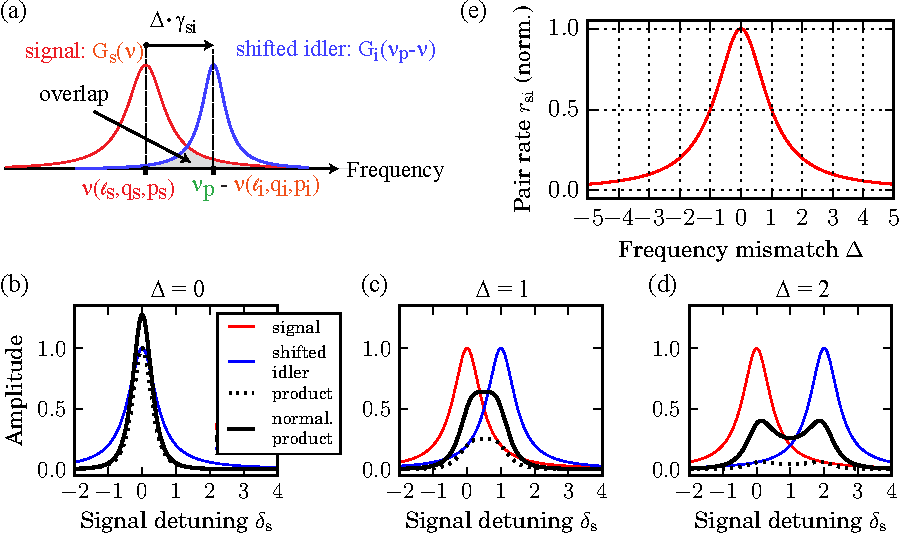
\includegraphics[scale=0.8]{pictures/teo_SPDC_spectrum/SPDC_spectrum_1.pdf}
	\caption{Frequency spectrum of parametric down-conversion below threshold. (a) The integrated product of the response functions $\tx{G}_\tx{s,i}(\nu) = |\mathcal{G}_\tx{s,i}(\nu)|^2$ of signal and idler in frequency space (see Eq.~\ref{eq:cavityresponse}) determines the parametric photon numbers $N_\tx{s,i}$ according to Eq.~\ref{eq:twophotonstate}. (b-d) The product of the signal $\tx{G}_\tx{s}(\nu)$ and the shifted idler $\tx{G}_\tx{i}(\gamma_\tx{si}\Delta + \nu (\ell_\textrm{s},\textrm{q}_\textrm{s},\textrm{p}_\textrm{s} ) +\nu (\ell_\textrm{i},\textrm{q}_\textrm{i},\textrm{p}_\textrm{i} ) -\nu) = \tx{G}_\tx{i}(\nu_\tx{p}-\nu)$ response functions ($\gamma_\tx{s}=\gamma_\tx{i} = \gamma_\tx{si}$ in this example) are plotted for various frequency mismatches $\Delta$ (see Eq.~\ref{eq:SPDCfrequ}). The black line shows the product normalized to a unity area. (e) The pair production rate ${r_\tx{si} \propto \left( 1+\Delta^2 \right)^{-1}}$ (see Eq.~\ref{eq:rategenbelow}) as a function on the frequency mismatch $\Delta$  is Lorentzian.} 
	\label{fig:spdc_spectrum}
\end{figure}

The oscillation threshold for the optical pump power $P^\tx{}_\textrm{th}\left( \delta_\textrm{p},\Delta\right)$ is then given by
\begin{align}
	 P_\textrm{th} \left( \delta_\textrm{p},\Delta\right) = \hslash 2 \pi \nu_\tx{p}  |\alpha^\tx{in}_\tx{p}|^2 = P_\textrm{0} \cdot \left(1 + 4 \delta_\textrm{p}^2 \right) \cdot \left(1 +  \Delta^2\right)   \,.
\label{eq:threshold}
\end{align}

In the limit of low gain, i.e far below threshold, we can iteratively solve the coupled wave equation for pump, signal, and idler with first-order perturbation theory for $|\alpha_\tx{p} g| / \gamma_\tx{s,i} \ll 1$. The noise power $S_\tx{s,i} (\nu)$ of the parametric photons at frequency $\nu$ in the resonator follows from 
\begin{alignat}{3}
	\avr{\hat{a}_\tx{s,i}\ssym{2} \left( \nu^\prime \right)\cdot \hat{a}_\tx{s,i} \left( \nu \right) } &= S_\tx{s,i} (\nu)  \cdot \delta(\nu - \nu^\prime) 
	\notag \\ 
	&=  \frac{2}{\pi \gamma_\tx{s,i}} \frac{ \tx{N}_\tx{p} }{\tx{N}_\tx{th}}  {{G}_\tx{s,i}\left( \nu + \nu (\ell_\textrm{s,i},\textrm{q}_\textrm{s,i},\textrm{p}_\textrm{s,i} ) \right)} \, {{G}_\tx{i,s} \left( \gamma_\tx{si} \Delta + \nu (\ell_\textrm{i,s},\textrm{q}_\textrm{i,s},\textrm{p}_\textrm{i,s} )  - \nu \right)}  \, .
\label{eq:spectrum}
\end{alignat} 

Vacuum fluctuations\footnote{For an evaluation of Eq.~\ref{eq:spectrum}, only the term $\avr{ \hat{\tx{f}}_\tx{s,i} \left( \nu\right) \hat{\tx{f}}_\tx{s,i} \ssym{2} \left( \nu\right) } = 2 \pi \gamma_\tx{s,i}$ gives a non-zero contribution.} $\hat{\tx{f}}_\tx{i} \left( \nu\right)$ of the idler mode drive the signal noise power, and visa verse. By integrating over the full frequency space, we get the number $N_\tx{s,i}$ of signal and idler photons in the resonator: 
\begin{align}
	N_\tx{s,i} &= \int S_\tx{s,i} (\nu) \, \tx{d} \nu = \frac{1}{\gamma_\tx{s,i}} \frac{ \tx{N}_\tx{p} }{\tx{N}_\tx{th}}  \frac{\gamma_\tx{s} \gamma_\tx{i} }{\gamma_\tx{si}} \frac{1}{1 + \Delta^2} \,  .  
	\label{eq:twophotonstate}
\end{align}

In parametric down-conversion, signal and idler are produced in pairs. Hence, we can define the rate of photon pair production ${r_\textrm{si}}{}$ in the resonator:
\begin{align}
	{r_\textrm{si}}{} = 2 \pi \,  \frac{\gamma^{}_\textrm{s} \gamma^{}_\textrm{i}}{\gamma^{}_\textrm{s} + \gamma^{}_\textrm{i}}  \frac{P^\tx{in}_\textrm{p}}{P_\textrm{th}\left( \delta_\textrm{p},\Delta \right)}  \, ,\quad (P^\tx{in}_\textrm{p} \ll P_\textrm{th})  \,.
\label{eq:rategenbelow}
\end{align}

The simultaneous generation of signal and idler  favors a description of parametric down-conversion in terms of temporal correlation functions \cite{Fekete2013,glauber1963,Michael2013,Ou1999,Scholz2009,Bocquillon2009,Bettelli2010,Luo2015}.


\FloatBarrier
\section{Experimental ontrol over the frequency mismatch $\Delta$}
In an ideal experiment, the pump light is switched off instantaneously. The outcoupled light from the cavity then results in a peak at the end of the pulse, since there is no longer destructive interference with the directly reflected pump light. The subsequent decay of the pulse corresponds to the cavity ring-down. An exponential fit of the cavity ring-down gives the pump bandwidth $\gamma_\tx{p}=\SI{34}{\MHz}$, which corresponds to critical coupling of the pump mode. 
\begin{figure}[htb]
  \centering
  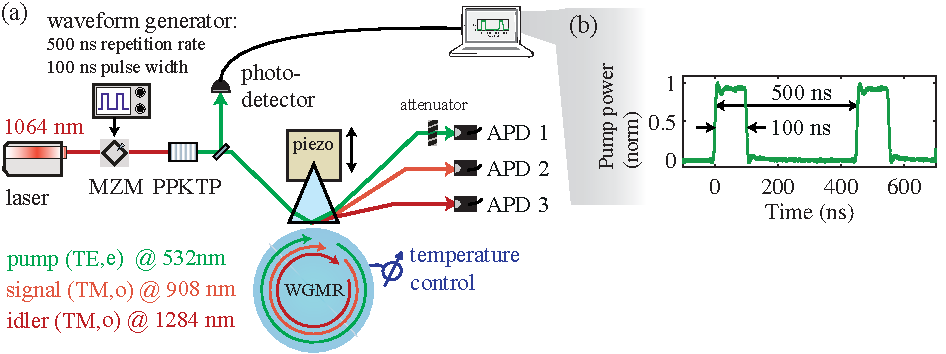
\includegraphics[scale=0.9]{pictures/exp_WGMR_detuning/WGMRsetup_pulsing4.pdf} 
\caption{Experimental setup for cavity-enhanced parametric down-conversion at pulsed excitation. (a) The pump laser frequency is repeatedly swept during \SI{100}{\ms} accross \SI{100}{\MHz} and then kept constant for another \SI{100}{\ms}. We use an amplitude modulator, i.e. a Mach-Zehnder modulator (MZM), to generate square pulses at the nanosecond scale from a continuous wave Nd:YAG laser at a wavelength of \SI{1064}{\nm}. (b) The pulses are frequency-doubled in a periodically poled potassium titanyl phosphate crystal (PPKTP) and monitored on a photodetector before the resonator. We use avalanche photodetectors for the detection of the signal photons below threshold.}
\label{fig:pulsingsetup}
\end{figure}
In the following, we discuss the generation rate of parametric photons (see Eq.~\ref{eq:rategenbelow}) depending on the phase matching of parametric down-conversion and the intracavity pump power. We show the signal count rates (see lower panels of Fig.~\ref{fig:pulsedcounts}(a,b)) depending on the resonator temperature. The pump laser was locked to the pump mode resonance frequency ($\delta_\tx{p}=0$). The pump laser absolute frequency then follows the temperature-induced frequency shifts\footnote{The approximate proportionality factors for frequency tuning by temperature are \SI{-27}{\MHz\per\milli\kelvin} for the pump mode and \SI{-6.3}{\MHz\per\milli\kelvin} for the parametric modes~\cite{Schlarb1994,Weis1985}.}. This frequency shift is proportional to the frequency mismatch of parametric down-conversion given by Eq.~\ref{eq:SPDCfrequ}. 

The maximal count rates in the lower panels of Fig.~\ref{fig:pulsedcounts}(a,b) are achieved for a zero frequency mismatch at discrete phase matching points. The two peaks in each trace correspond to adjacent longitudinal parametric conversion channels. The non-Lorentzian profiles (see Eq.~\ref{eq:rategenbelow}) additionally indicate the presence of other conversion channels, which have not been blocked with bandpass filters for this measurement \cite{Michael2014}.

\begin{figure}[htb]
  \centering
  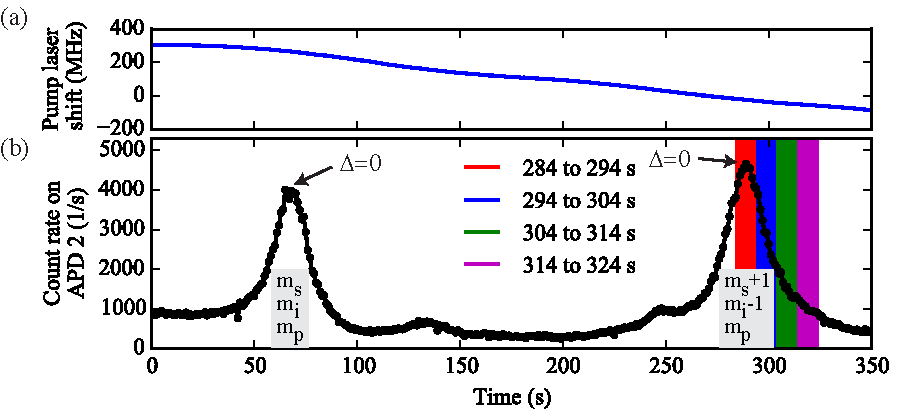
\includegraphics[scale=0.8]{pictures/exp_WGMR_detuning/SPDC_detuning_tempshift_1.pdf} 
\caption{Temperature-dependent phase matching of parametric down-conversion below threshold. (a) The signal photons are recorded during the hold phase of the laser (see Fig.~\ref{fig:pulsingsetup}) with the laser frequency being locked to the pump mode resonance frequency ($\delta_\tx{p} = 0, \Delta =2 \cdot \left( \nu (\ell_\textrm{p},\textrm{q}_\textrm{p},\textrm{p}_\textrm{p}) - \nu (\ell_\textrm{s},\textrm{q}_\textrm{s},\textrm{p}_\textrm{s}) - \nu (\ell_\textrm{i},\textrm{q}_\textrm{i},\textrm{p}_\textrm{i})\right) / \gamma_\tx{si} $). (a) We continuously increasing the resonator temperature on the time scale of seconds while measuring the detuning of the pump laser. An increase in the resonator temperature corresponds to a decrease in the resonance frequencies $\nu (\ell_\textrm{p,s,i},\textrm{q}_\textrm{p,s,i},\textrm{p}_\textrm{p,s,i})$ and hence to a decrease in the frequency mismatch of parametric down-conversion $\Delta$ (see  Eq.~\ref{eq:SPDCfrequ}). (b) The pump mode bandwidth was $\gamma_\tx{p}=\SI{66666}{\MHz}$. The single photon rates on the time scale of nanoseconds are shown in Fig.~\ref{fig:pulsedcountsnano} for the respective time slots.}
	\label{fig:pulsedcounts}
\end{figure}

\begin{figure}[htb]
  \centering
  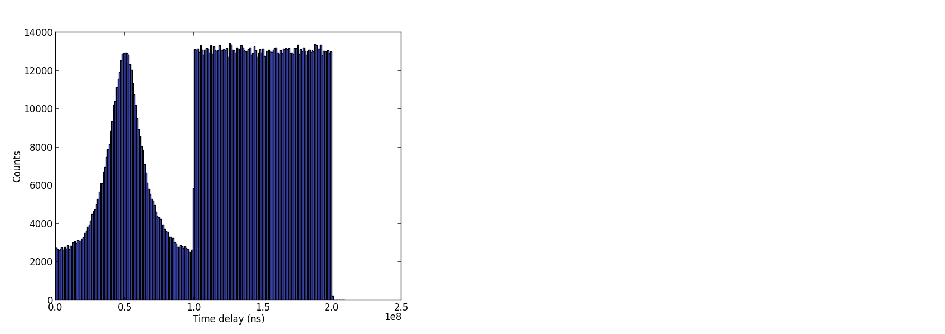
\includegraphics[scale=0.8]{pictures/exp_WGMR_detuning/SPDC_frequ_sweep.pdf} 
\caption{Count rates depending on the pump frequency for different phase-matching temperatures. (a) We sweep the pump laser frequency in \SI{100}{\ms} in a $100~\tx{MHz}$-intervall symmetrically around the pump mode (see sweep phase in Fig.~\ref{fig:pulsingsetup}) and measure the reflected power $P^\tx{refl.}_\tx{p}$ (the cavity instensity response ${G}_\tx{p} (\nu_\tx{p})$ follows from  ${G}_\tx{p}(\nu_\tx{p}) \propto 1 - P^\tx{refl.}_\tx{p} / P^\tx{in}_\tx{p}$. (b) Depending on the phase-matching temperatures (see Fig.~\ref{fig:pulsedcounts}), we measure a lower maximal count rate and a shift of the count rate maximum to the right-hand side. (c) The signal count rates normalized to the intracavity pump power $P_\tx{p} = \hbar \, \nu_\tx{p} |\hat{\alpha}|^2 \propto {G}_\tx{p} (\nu_\tx{p})$ shows the shift of the phase-matched ($\Delta=0$) pump laser frequency $\nu_p$ relative to the pump resonance frequency $\nu (\ell_\tx{p},\tx{q}_\tx{p},\tx{p}_\tx{p})$. }
	\label{lockingsignal}
\end{figure}


Parametric down-conversion in the resonator is driven by an exponential loading curve of the internal pump. The signal counts in Fig.~\ref{fig:pulsedcountsnano} exhibit an exponential loading curve similar to the pump, but with a time constant determined by the overlap of the parametric modes depending on the frequency mismatch $\Delta$ (see Fig.~\ref{fig:spdc_spectrum}). The highest photon rates with the longest rise times are achieved for a zero frequency mismatch (red traces: \SIrange[range-units = single]{284}{294}{\s} in Fig.~\ref{fig:pulsedcountsnano}(a) and \SIrange[range-units = single]{124}{154}{\s} in Fig.~\ref{fig:pulsedcountsnano}(b)). At non-zero frequency mismatch $\Delta$, photon rates are decreased and rise time is increased. We attribute the latter to the higher bandwidth of the parametric frequencies at non-zero detuning.
\begin{figure}[htb]
	\centering
	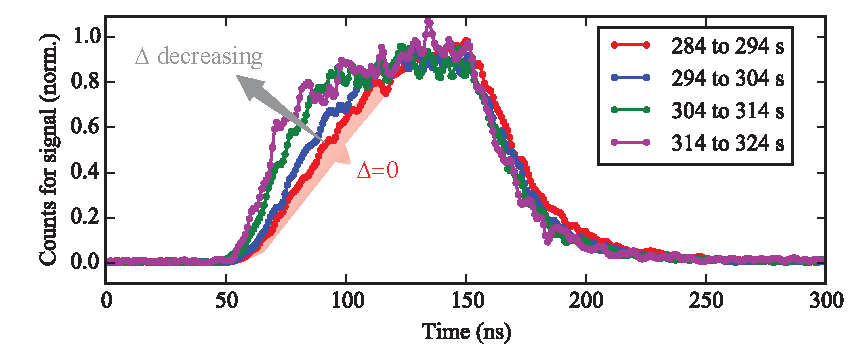
\includegraphics[scale=0.8]{pictures/exp_WGMR_detuning/SPDC_detuning_pulses_1.pdf} 
	\caption{Signal photon count rates at pulsed excitation. The signal counts are recorded during the hold phase of the laser frequeny (see Fig.~\ref{fig:pulsingsetup}). Each trace corresponds to a different temperature-induced frequency mismatch $\Delta$ of parametric down-conversion shown in Fig.~\ref{fig:pulsedcounts}. At the beginning of the pulses, we observe shorter rise times of the count rates for an decreased frequency mismatch $\Delta$. The unmodified cavity ring-down is observed at the end of the pulses leading to a signal bandwidth of ${\gamma_\tx{s}=\SI{7.4}{\MHz}}$.}
	\label{fig:pulsedcountsnano}
\end{figure}

At the end of the pulse, the pump light quickly couples out from the resonator. This region corresponds to the cavity ring-down where the rate of the signal photons is solely determined by the bandwidth of the signal mode. The first part of the pulse in Fig.~\ref{fig:pulsedcountsnano} already gives us an exponentially rising single photon wave packet. The end part of the pulse, however, adds an exponentially decreasing tail to each single photon temporal mode due to cavity ring-down of each photon.

\FloatBarrier
\section{References}
	\bibliographystyle{apsrev4-1}
	\bibliography{MyCollection}
%	

%\begin{thebibliography}{10}
%
%\newcommand{\enquote}[1]{``#1''}
%\bibitem{Specht2011}
%H.~P. Specht, C.~N\"{o}lleke, A.~Reiserer, M.~Uphoff, E.~Figueroa, S.~Ritter
%  and G.~Rempe.
%\newblock \emph{{A single-atom quantum memory}}.
%\newblock Nature \textbf{473}, 190 (2011).
%\end{thebibliography}

\end{document}

